\documentclass{standalone}
% \usepackage{tikz}
\usepackage{pgfplots}
% \usepackage{amsmath}
% \DeclareMathOperator{\Real}{Re}
% \DeclareMathOperator{\Imag}{Im}
\begin{document}
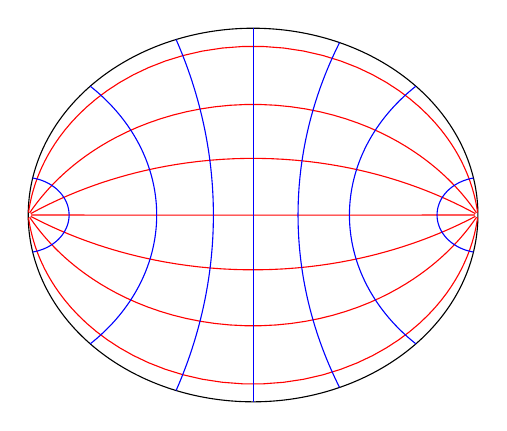
\begin{tikzpicture}
\begin{axis}[axis lines=none]

\addplot[domain=0:360,samples=360] ({cos(x)},{sin(x)});

\foreach \d in {0.1,0.5, 1, 1.57, 2.16, 2.64,3.04}
    \addplot[domain=-5:5,samples=100,color=red] ({ (exp(x)^2 - 1)/(exp(x)^2 + 2*exp(x)*sin(\d r) + 1) },{ (-2*exp(x)*cos(\d r))/(exp(x)^2 + 2*exp(x)*sin(\d r) + 1) });

\foreach \xx in {0.1, 0.4, 0.7, 1, 1.5, 2.5 , 10}
    \addplot[domain=0:180,samples=100,color=blue] ({ (\xx^2 - 1)/(\xx^2 + 2*\xx*sin(x) + 1) },{ (-2*\xx*cos(x))/(\xx^2 + 2*\xx*sin(x) + 1) });

\end{axis}
\end{tikzpicture}
\end{document}
